%----------------------------------------------------------------------------------------
%	CHAPTER 2
%----------------------------------------------------------------------------------------
%\chapterimage{}
\cleardoublepage
\chapterimage{chap_head.png}
\chapter{Fun with LEDs}

\section{Overview}\index{Overview}
In this section you'll learn about Light Emitting Diodes (LED) and how to turn it on using different methods.


\section{Component Introduction}\index{Component Introduction!LEDs}
Before diving into making circuits, we will first learn about the components that we are going to use and how to select the right component.

\subsection{Resistors}
Resistor is a passive electric component that resists the flow of current through it. They are used in almost all electrical and electronic circuits and systems. The resistance of a resistor in measured in ohms (\textOmega).
An ohm is the resistance that occurs when one ampere (A) of current flows through a resistor with potential (or voltage) drop of one volt (V) across it's terminal.
\begin{figure}[!htp]
    \centering
    \begin{circuitikz}[scale = 2]
        \draw[very thick] (0,0) to[resistor, color = red] (2,0);
    \end{circuitikz}
    \caption{Resistor Symbol}
    \label{fig:resistor_symbol}
\end{figure}

\subsubsection{Ohm's Law}
Ohm's law state that the current through a resistor is directly proportional to the voltage applied across it.
\begin{align*}
    I \propto V \\
    \Longrightarrow
    R = \frac{V}{I} (\Omega)
\end{align*}
\subsubsection{Reading Resistor Value}
To read the value of resistance, first you need to know it's tolerance, this is known as E-series. E-24 series resistors have 5\% 
tolerance, whereas E-48 has 2\%. Once, you know the tolerance, you need to identify whether it's 4-Bands or 5-Bands. 
The last band represents tolerance (from the figure \ref{fig:res_color_code} you can tolerance band for 5\%) and the second last 
is the exponential power of 10. So, if a 4-Bands resistor has a color code of Brown, Green, Orange and Gold it's value will be -
\begin{align*}
    R_{Value} &= (1_{Brown}  5_{Green}) \times 10^{(3_{Orange})} \pm 5 \% \\
    R_{Value} &= (15) \times 10^{(3)} \pm 5\% \\
    R_{Value} &= 15\si{\kohm} \pm 5\% \\
\end{align*} 
\begin{figure}[!htb]
    \centering
    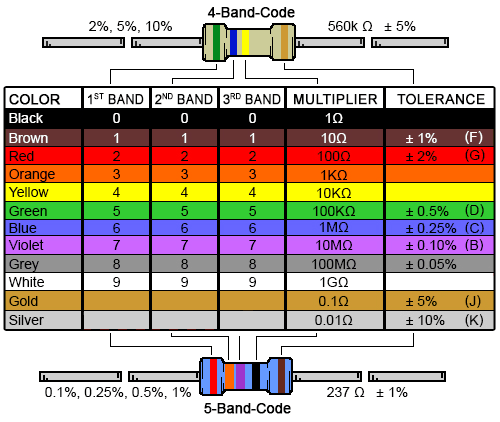
\includegraphics[width=0.8\textwidth]{Components/resistor-color-code.png}
    \caption{Resistor Color Code}
    \label{fig:res_color_code}
\end{figure}

\subsection{Light Emitting Diode}
Light emitting diodes (LEDs) are semiconductor devices that emit lights of different wavelength depending on the substrate semiconductor material used when an electric current is applied. The color of light emitted depends on the amount of energy required by the electrons to cross the band gap of the semiconductor. Since, LEDs are basically a PN junction diode, they allow current flow only in one direction.

\begin{figure}[!htp]
    \centering
    \begin{circuitikz}[scale = 2]
        \draw[very thick] (0,0) to[full led, color = red] (2,0);
    \end{circuitikz}
    \caption{LED Symbol}
    \label{fig:led_symbol}
\end{figure}

\subsubsection{Determining the pins of the LED}
There are multiple ways to determine the anode and cathode of an LED:
\begin{enumerate}
    \item Looking at the LED pins (or legs). The longer leg is anode and the shorter cathode. But sometimes the legs could be trimmed, therefore, you can use this method for new LEDs only.
    \item Locate a flat edge on the LED. The pin close to flat edge is cathode.
    \item By looking inside the LED, the bigger conductor (flag shaped) is the cathode.
    \item By using multi-meter in continuity mode, only is one direction the LED will turn on (or the resistance in one direction will be smaller than in the other).
\end{enumerate}

\begin{figure}[!htp]
    \centering
    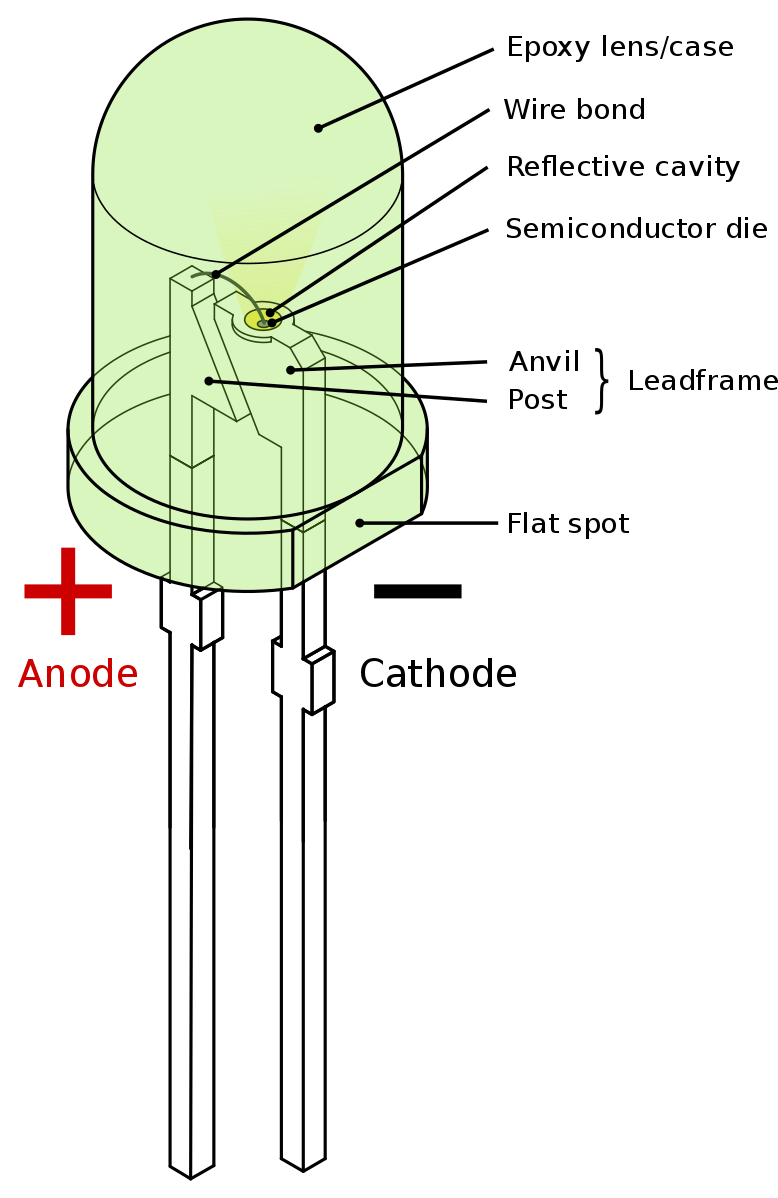
\includegraphics[width=0.4\textwidth]{Components/LED-code.png}
    \caption{LED}
    \label{fig:led_code}
\end{figure}

\subsection{Breadboard}
A breadboard in a rectangular plastic board with a bunch of tiny holes in it. There's strip of metal inside the plastic. Most through hole components have pin spacing of 2.54mm, therefore, the holes have the same spacing between them. You can easily insert electrical components in these holes. There is also a deep grove in the middle, indicating the break in the connection. Some breadboard have two strips of holes (also called rails) along the long edges of the breadboard. They are used for power rails, with strip of metal inside.
\begin{figure}[!htp]
    \centering
    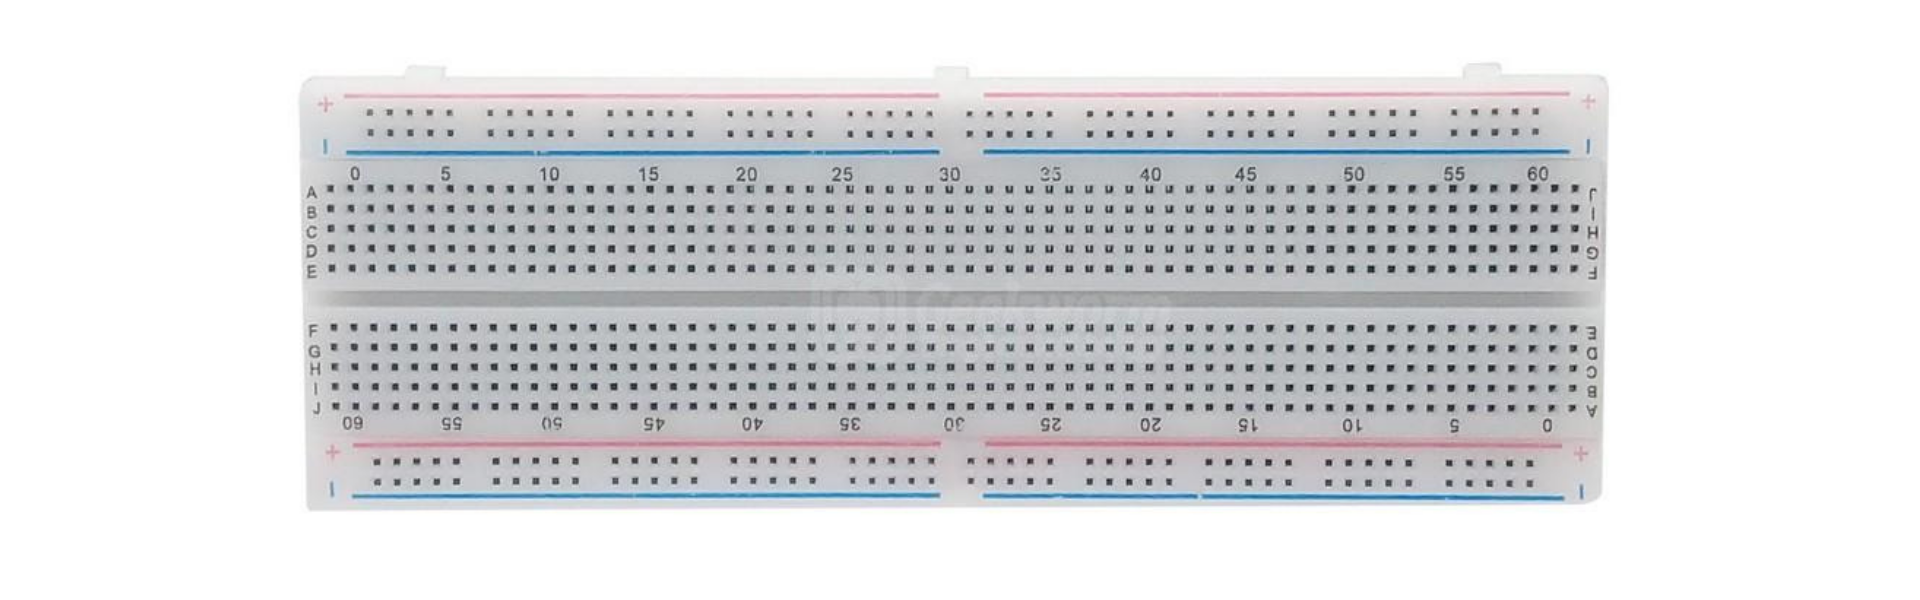
\includegraphics[width=\textwidth]{Components/breadboard.png}
    \caption{Breadboard}
    \label{fig:breadboard_code}
\end{figure}
A breadboard is used to prototype an electronic circuit. The connection on breadboard are not permanent and can be removed easily. This makes breadboard great for beginners who are new to electronics but the connections are not as reliable as soldered connections.

\subsection{Breadboard Power Supply}
A power supply is a hardware component that provides electricity to power devices like computer, fridge, lights and much more. The breadboard power supply of type linear DC to DC. A linear power supply has two major components, a linear regulator and filtering capacitors.
\begin{figure}[!htp]
    \centering
    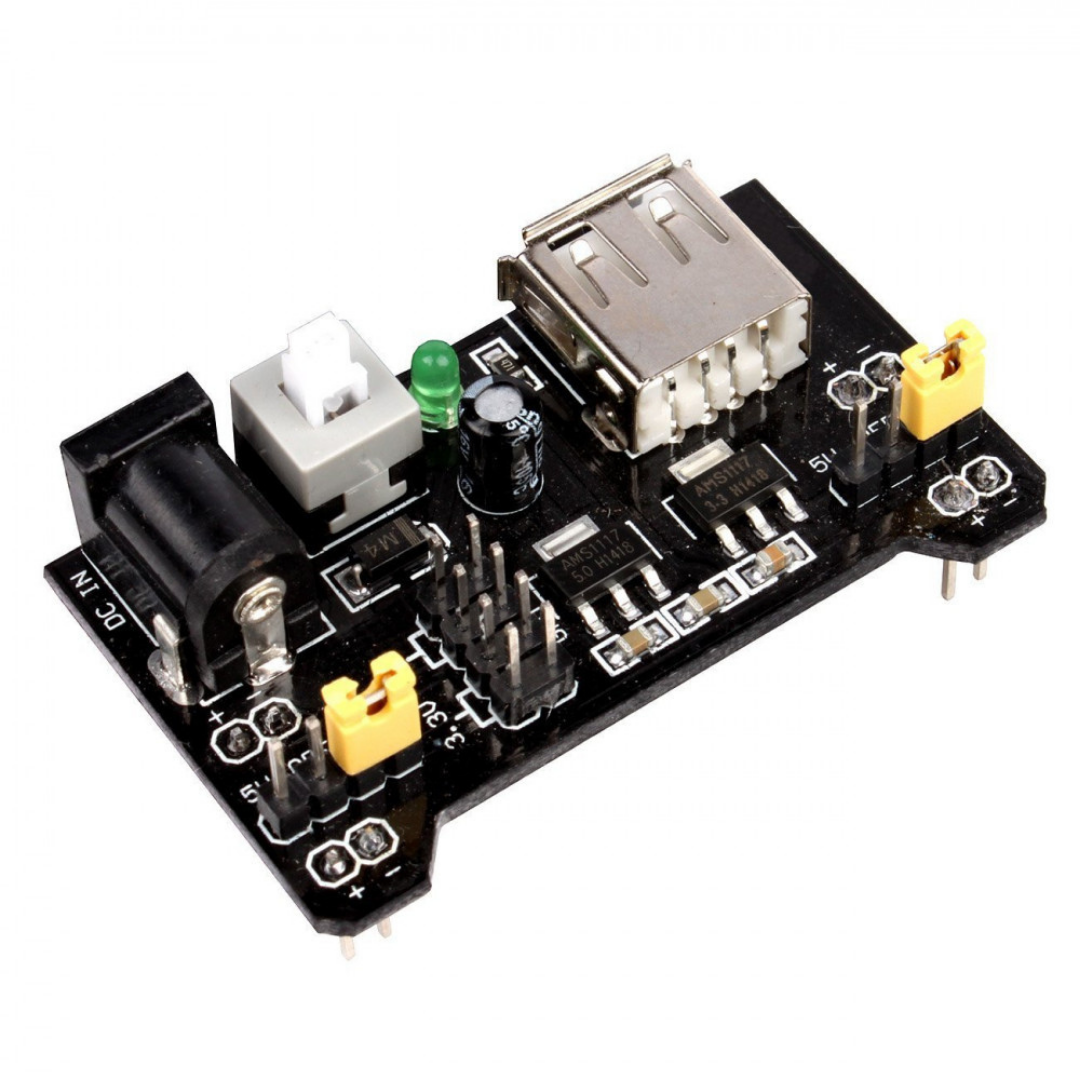
\includegraphics[width=0.6\textwidth]{Components/breadboard-power-supply.png}
    \caption{Breadboard Power Supply}
    \label{fig:breadboard_ps_code}
\end{figure}
The breadboard power supply can provide constant 3.3V or 5V and is compatible with the breadboard power rails, i.e., you can directly plug in on top of the breadboard to have voltage across the power rails.
The input voltage or power can be provided through the DC barrel jack (for 6-12V) or through the USB connector (5V).

\begin{figure}[!htp]
    \centering
    \begin{circuitikz}[scale = 2]
        \draw
            [very thick] (0,2) to[battery, color = red] (0,0)
            (0.2,1.2) node{$+$}
            (0.2,0.8) node{$-$};
    \end{circuitikz}
    \caption{Battery Symbol}
    \label{fig:battery_symbol}
\end{figure}

\subsubsection{Calculating power dissipation}
To calculate the power dissipation across the voltage regulator, we need to determine the output current. For linear regulator the input and output current remains same and the power difference is dissipated through the voltage regulator.

Example: We need 200mA current at 3,3V output, and the input power supply is of 9V. Then,
\begin{align*}
    P_{out} &= 3.3V \times 0.2A = 0.66W \\
    P_{in} &= 9V \times 0.2A = 1.8W \\
    P_{reg} &= P_{in} - P_{out} \\
        &= 1.8 - 0.66 \\
        &= 1.14W \\
    \eta &= \frac{P_{out}}{P_{in}} \times 100\\
        &= 36.67 \%
\end{align*}

\subsection{Push Button}
Push button is use to control or provide input to the circuit. It is normally open and only when you press it the current will flow through it. And when released, the current will stop flowing. Push button have mechanical contacts, so when you press or release it, it doesn't instantaneously make or release contact. It bounces back and forth before making a firm connection.
\begin{figure}[!htp]
    \centering
    \begin{circuitikz}[scale = 2]
        \draw[very thick] (0,0) to[push button, color = red] (2,0);
    \end{circuitikz}
    \caption{Push Button Symbol}
    \label{fig:pb_symbol}
\end{figure}
\begin{figure}[!ht]
    \centering
    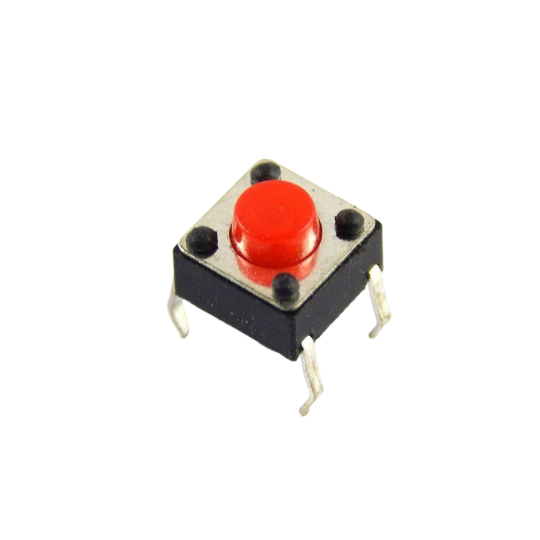
\includegraphics[width=0.4\textwidth]{Components/push-button.png}
    \caption{Tactile Push Button}
    \label{fig:pb_code}
\end{figure}

\subsection{Potentiometer}
A potentiometer (pot) is a variable resistor and comes in different packages, size and values. They generally have 3 terminals. And the resistance between the outer most terminals is equal to the maximum resistance of the potentiometer and the resistance between middle and any outer pin can vary from 0 to the total resistance of potentiometer.
\begin{figure}[!htp]
    \centering
    \begin{circuitikz}[scale = 2]
        \draw[very thick] (0,0) to[american potentiometer, color = red] (2,0);
    \end{circuitikz}
    \caption{Potentiometer Symbol}
    \label{fig:pot_symbol}
\end{figure}
\begin{figure}[!ht]
    \centering
    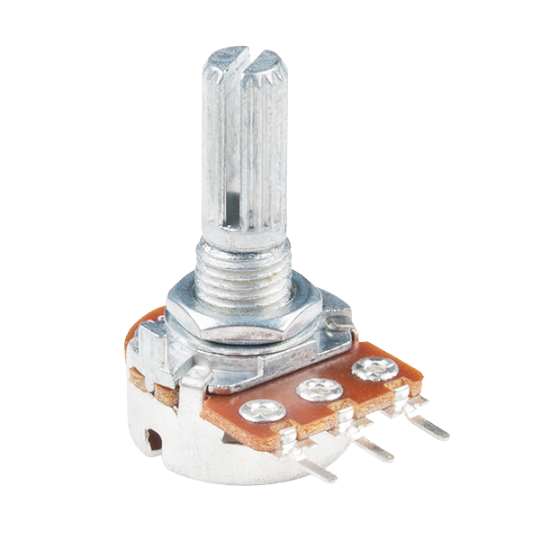
\includegraphics[width=0.5\textwidth]{Components/potentiometer.png}
    \caption{Potentiometer}
    \label{fig:pot_code}
\end{figure}

\subsection{Circuit}
A circuit is a closed loop that provides path for current to flow. Circuit must have a path that start and end at the same component, or in order words must form a loop. Electronic circuits operates at low voltages.
\begin{figure}[!htp]
    \centering
    \begin{circuitikz}[scale = 2]
        \draw
            [blue] (0,0) to[short] (3,0)
            (0,1) to[full led, color=red] (3,1)
            (3,0) to[R] (3,1)
            (0,1) to[battery, color=red] (0,0);
    \end{circuitikz}
    \caption{Simple Circuit}
    \label{fig:simple_circuit}
\end{figure}

A circuit has broadly the following components -
\begin{itemize}
    \item Power source\/supply
    \item Load (Light, led, motor etc)
    \item Path\/wire (conductive path providing current flow)
\end{itemize}
Apart from these, a circuit can have more complex design.


\clearpage

% Lesson starts here
\section{Lesson 1: Lighting up an LED}\index{Lesson 1: Lighting up an LED}
\subsection{Objective}
In this activity you'll learn how to turn on an LED
\subsection{Components Required}
\begin{enumerate}
    \item Breadboard Power Supply $\times$ 1
    \item 9V Battery $\times$ 1 
    \item 9V Battery Connector $\times$ 1
    \item Breadboard $\times$ 1
    \item 5mm Red LED $\times$ 1
    \item 220$\Omega$ resistor $\times$ 1
    \item Male to Male Jumper Wires $\times$ 2
\end{enumerate}
\subsection{Circuit}
\begin{figure}[!htp]
    \centering
    \begin{subfigure}[b]{0.4\textwidth}
        \centering
        \begin{circuitikz}[scale = 2]
            \draw[very thick]
                (0,0) to[short] (2,0)
                (0,1) to[full led, color=red] (2,1)
                (2,0) to[R, l^=$R_s (220\Omega)$] (2,1)
                (0,1) to[battery, color=red, l_=$5V$] (0,0);
        \end{circuitikz}
        \caption{Circuit A}
    \end{subfigure}
    \hfill
    \begin{subfigure}[b]{0.4\textwidth}
        \centering
        \begin{circuitikz}[scale = 2]
            \draw[very thick]
                (0,0) to[short] (2,0)
                (0,1) to[R, l^=$R_s (220\Omega)$] (2,1)
                (2,1) to[full led, color=red] (2,0)
                (0,1) to[battery, color=red, l_=$5V$] (0,0);
        \end{circuitikz}
        \caption{Circuit B}
    \end{subfigure}
    \caption{Simple LED Circuits}
    \label{fig:simple_led_circuit}
\end{figure}
Throughout this guide we'll be using these symbols for power supply.
\begin{figure}[!htp]
    \centering
    \begin{subfigure}[b]{0.4\textwidth}
        \centering
        \begin{circuitikz}[scale = 2]
            \draw
                (0,1) to[empty led, color=red] (0,0)
                (0,0) node[ground] {}
                (0,1) to[R, l^=$R_s (220\Omega)$] (0,2)
                (-0.2,2) -- node[anchor=south] {5V} (0.2,2);
        \end{circuitikz}
        \caption{Circuit A}
    \end{subfigure}
    \hfill
    \begin{subfigure}[b]{0.4\textwidth}
        \centering
        \begin{circuitikz}[scale = 2]
            \draw
                (0,2) to[empty led, color=red] (0,1)
                (0,0) node[ground] {}
                (0,1) to[R, l^=$R_s (220\Omega)$] (0,0)
                (-0.2,2) -- node[anchor=south] {5V} (0.2,2);
        \end{circuitikz}
        \caption{Circuit B}
    \end{subfigure}
    \caption{Simplified LED Circuits}
    \label{fig:led_circuit}
\end{figure}
\subsection{Circuit Explanation}
If we look at the graphs in the data-sheet of RED led\cite{tlur640}, the forward current through the led ($I_F$) is typically 
in between \SI{10}{mA} to \SI{20}{mA} and the voltage drop ($V_F$) across it is \SI{2}{V}. If we directly connect the LED across 
\SI{5}{V} supply it will burn out due to excessive power. Therefore, we need a resistor in series with the LED to drop the voltage. 
This resistor is referred as the current-limiting resistor. If you look at the figure \ref{fig:simple_led_circuit} both the circuits 
A \& B are same because in series circuits the current remains same across all the components.

To calculate the series resistance ($R_S$) we'll use Ohm's law:
We'll take the average value for $I_F$
\begin{align*}
    V &= I \times R \\
    R_S &= \frac{V_{5v} - V_F}{I_F} \\
        &= \frac{5V - 2V}{15mA} \\
        &= \frac{3 \times 1000}{15} \\
    R_S &= \SI{200}{\Omega}
\end{align*}
Since, in the kit a \SI{220}{\ohm} is available, we will use that. If we calculate the current using a \SI{220}{\ohm} resistor, it will $3 \div 220 = \SI{0.0136}{\ampere} = \SI{13.6}{\mA}$ which is in the range provided by the data-sheet.
\subsection{Circuit Picture}
\begin{figure}[!htp]
    \centering
    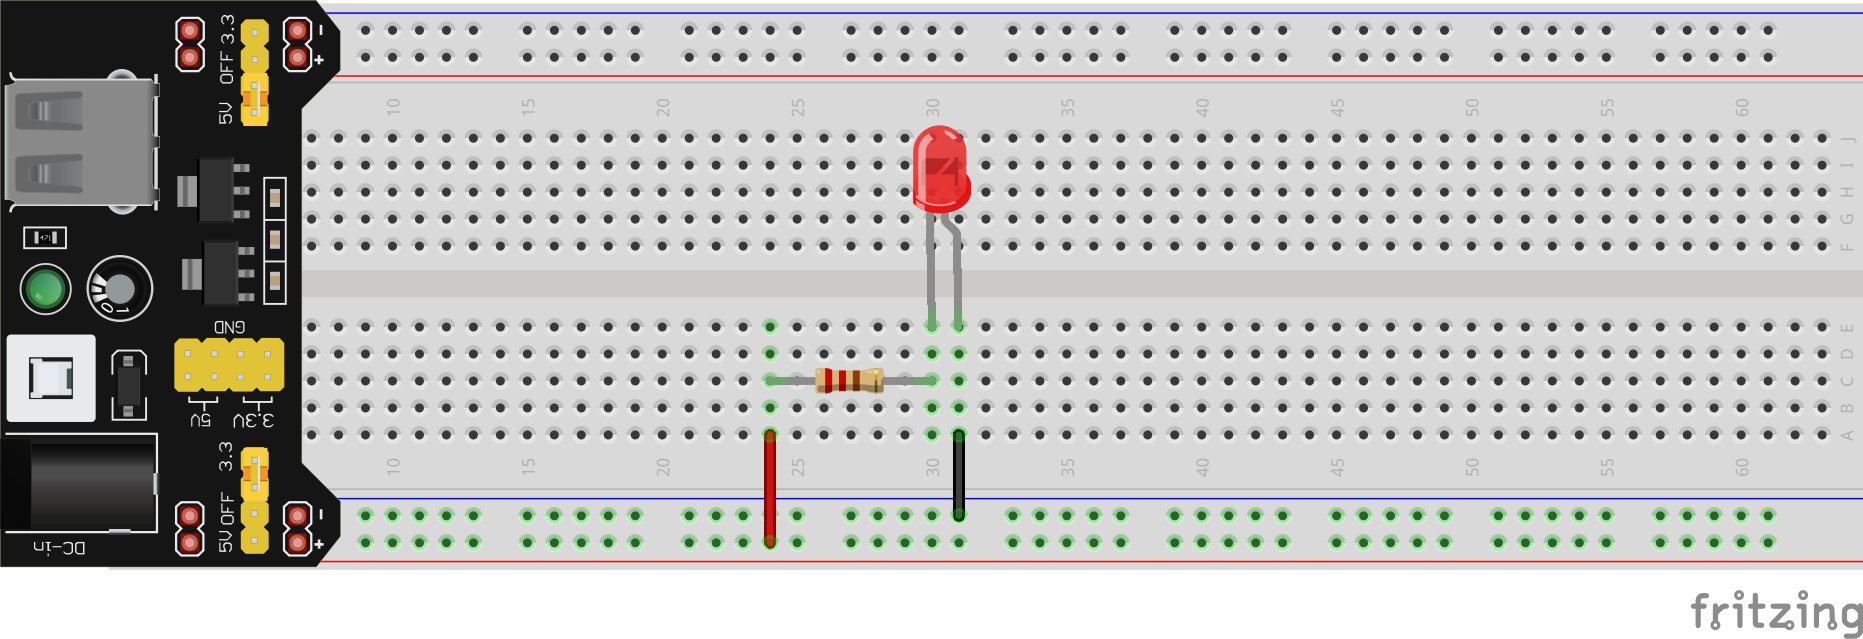
\includegraphics[width=0.8\textwidth]{lesson_circuits/L1/lesson_1.png}
    \caption{Simple Circuit Breadboard Schematic}
    \label{fig:sc_bb}
\end{figure}
\begin{figure}[!htp]
    \centering
    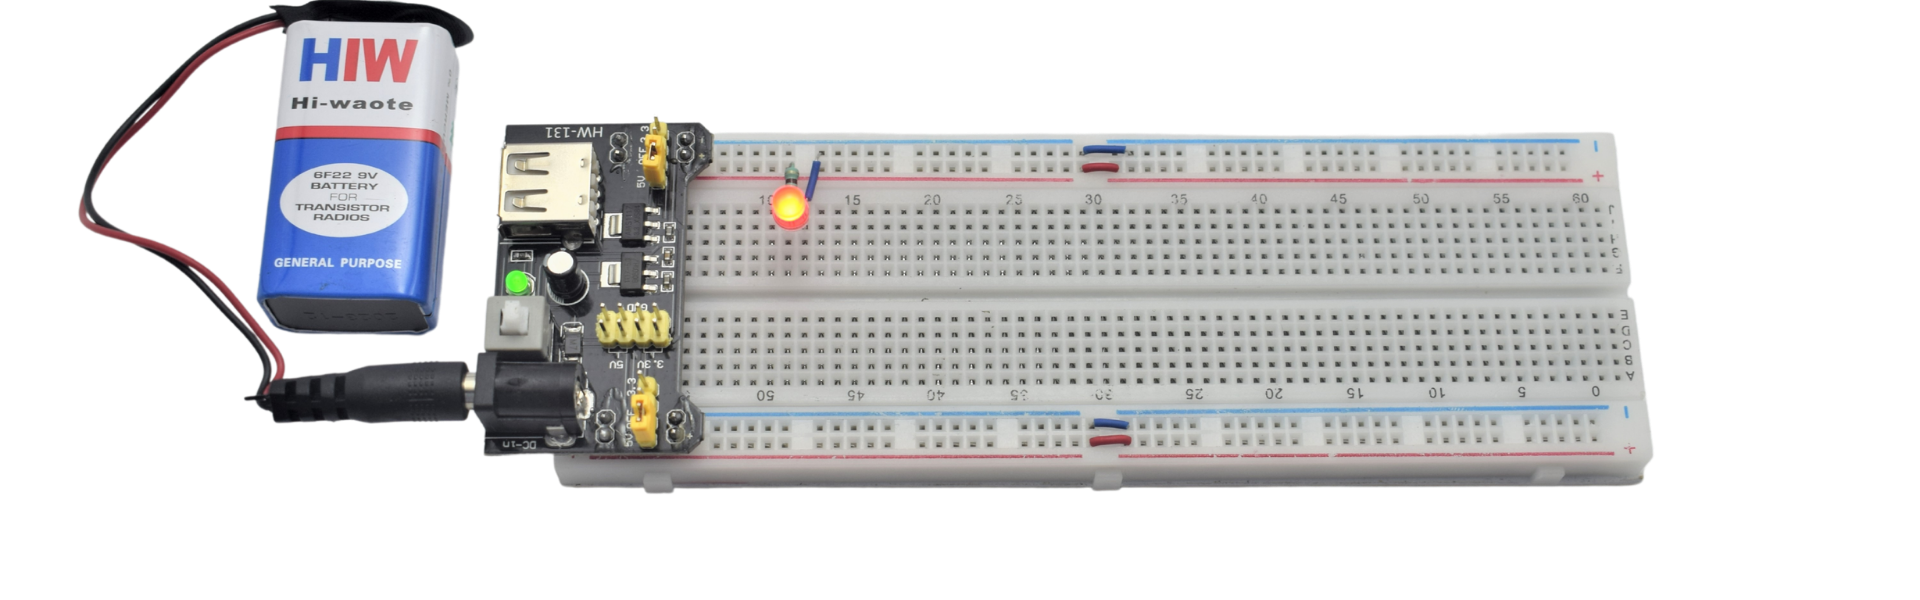
\includegraphics[width=\textwidth]{lesson_circuits/L1/L1-A.png}
    \caption{Simple Circuit on Breadboard}
    \label{fig:sc_obb}
\end{figure}



\clearpage
\section{Lesson 2: Lighting up an LED by pressing a Switch}
\subsection{Objective}
In this activity we'll turn on the led using a push button.
\subsection{Components Required}
\begin{enumerate}
    \item Breadboard Power Supply $\times$ 1
    \item 9V Battery $\times$ 1 
    \item 9V Battery Connector $\times$ 1
    \item Breadboard $\times$ 1
    \item 5mm Red LED $\times$ 1
    \item 220$\Omega$ resistor $\times$ 1
    \item Male to Male Jumper Wires $\times$ 2
    \item Push Button $\times$ 1
\end{enumerate}
\subsection{Circuit}
\begin{figure}[!htp]
    \centering
    \begin{circuitikz}[scale = 2]
        \draw
            (0,1) to[empty led, color=red] (0,0)
            (0,0) node[ground] {}
            (0,1) to[R, l^=$R_s (220\Omega)$] (0,2)
            (0,3) to[push button] (0,2)
            (-0.2,3) -- node[anchor=south] {5V} (0.2,3);
    \end{circuitikz}
    \caption{Push Button Circuit}
    \label{fig:pb_led_circuit}
\end{figure}
\subsection{Circuit Explanation}
This circuit is similar to the one we made previously, except for the fact that we have a push button in series. The button is normally open, meaning no current flows through the circuit (no complete loop or path) and when we press the button the path is complete and LED will turn on.
\subsection{Circuit Photo}
\begin{figure}[!htp]
    \centering
    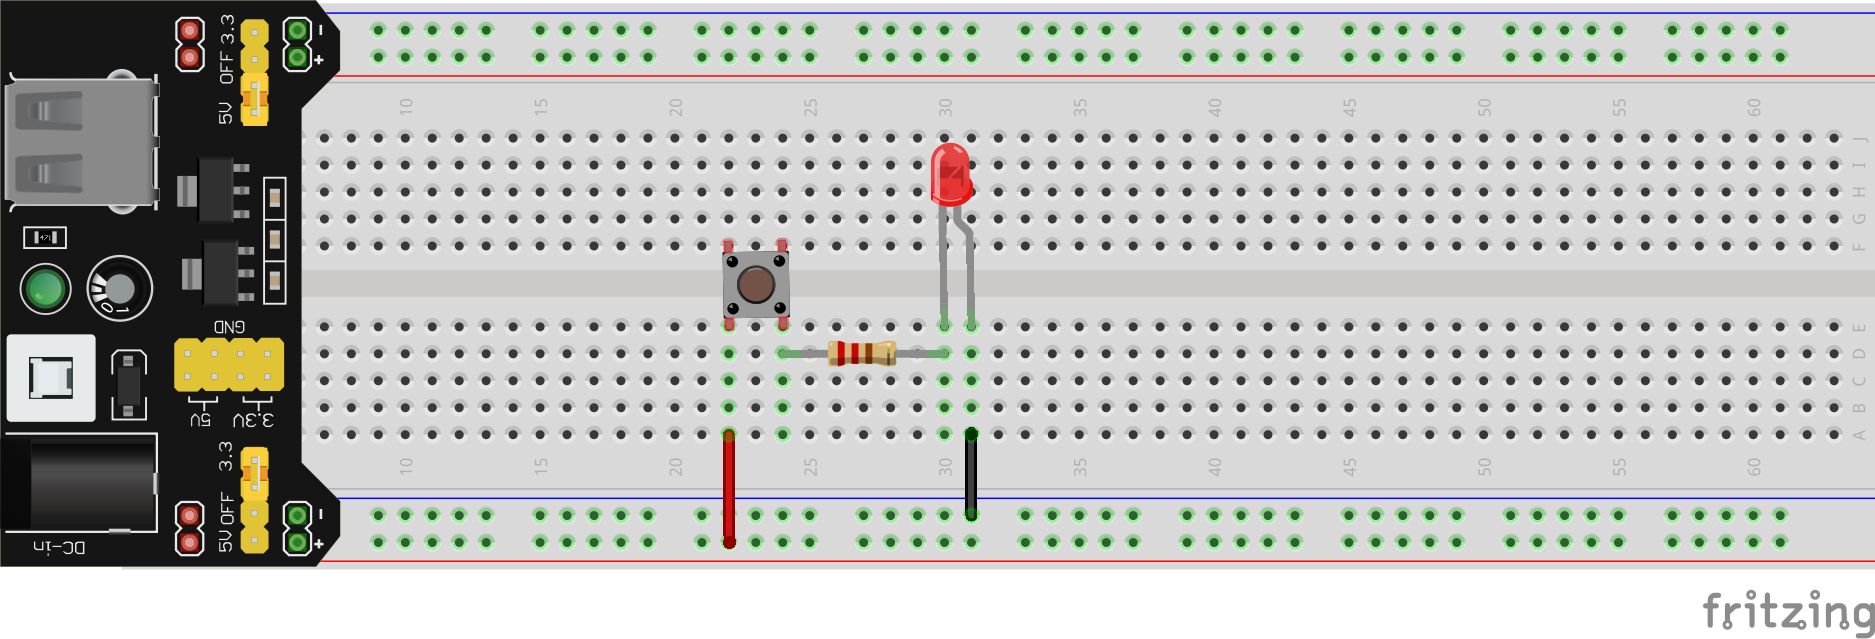
\includegraphics[width=0.8\textwidth]{lesson_circuits/L2/lesson_2.png}
    \caption{Breadboard Schematic}
    \label{fig:pb_led_sch}
\end{figure}
\begin{figure}[!htp]
    \centering
    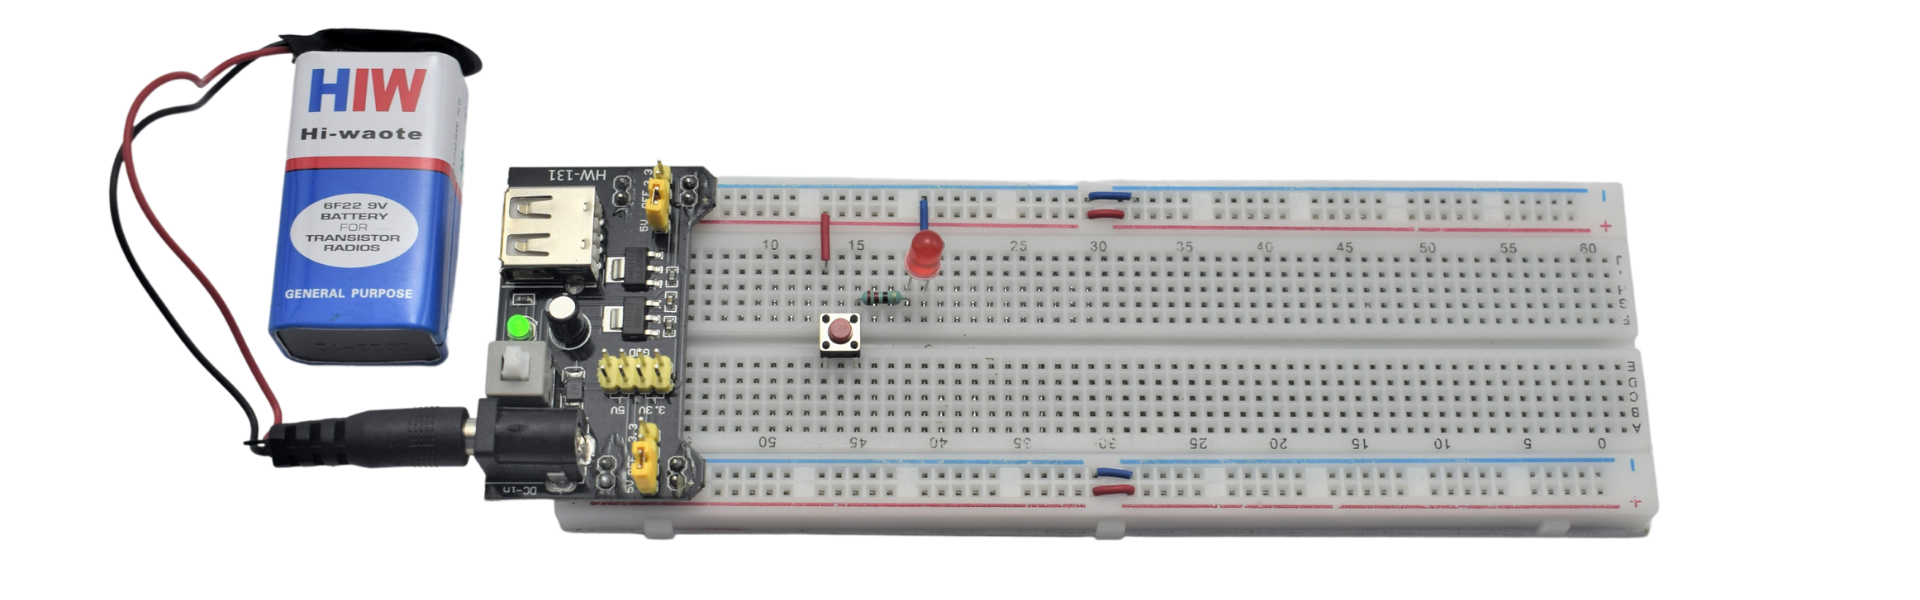
\includegraphics[width=\textwidth]{lesson_circuits/L2/L2-A.png}
    \caption{LED Off, Switch Open}
    \label{fig:pb_led_offl}
\end{figure}
\begin{figure}[!htp]
    \centering
    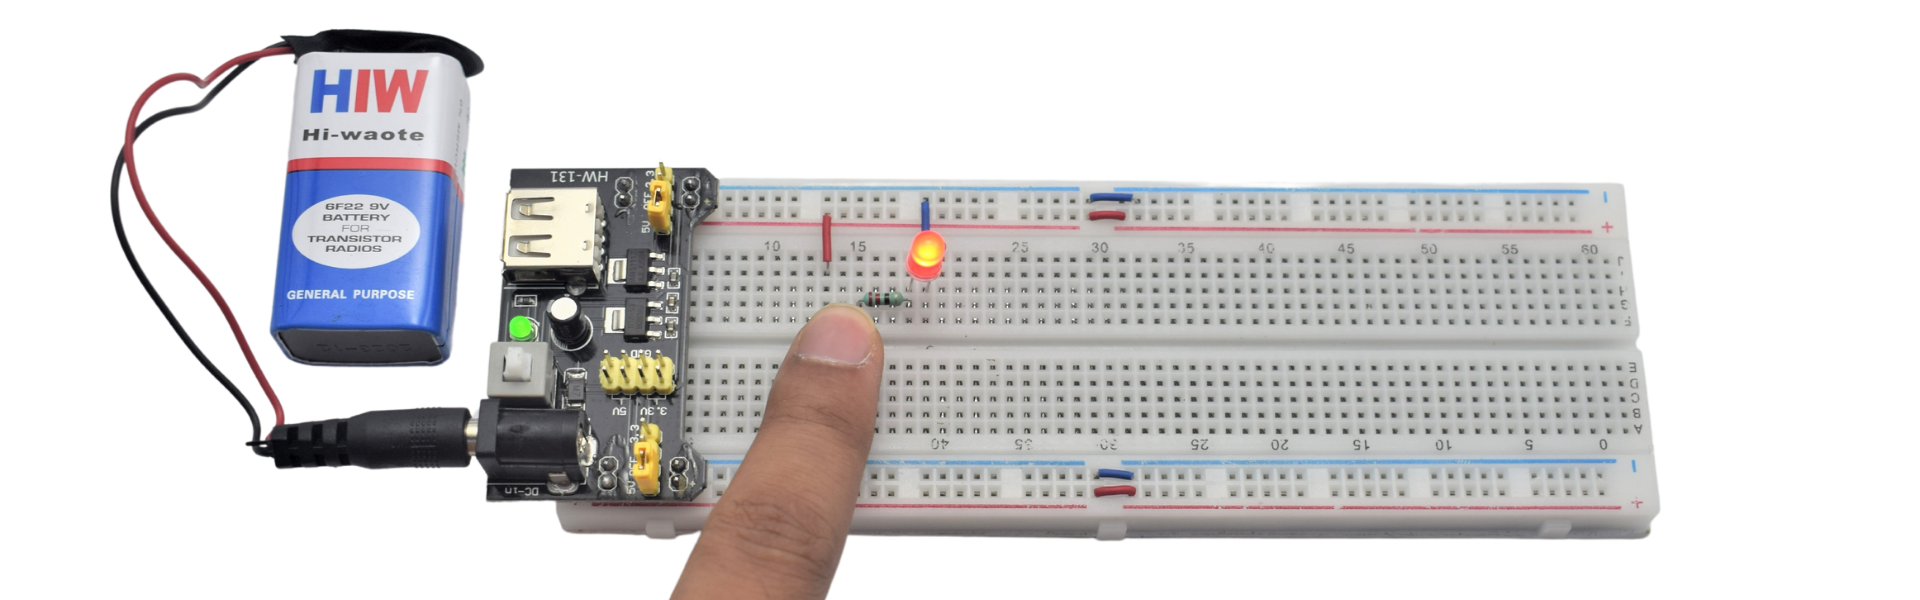
\includegraphics[width=\textwidth]{lesson_circuits/L2/L2-B.png}
    \caption{LED On, Switch Closed/Pressed}
    \label{fig:pb_led_onl}
\end{figure}



\clearpage
\section{Lesson 3: Controlling LED brightness using a Potentiometer}
\subsection{Objective}
In this activity, we'll control the LED brightness/intensity with help on a potentiometer.
\subsection{Components Required}
\begin{enumerate}
    \item Breadboard Power Supply $\times$ 1
    \item 9V Battery $\times$ 1 
    \item 9V Battery Connector $\times$ 1
    \item Breadboard $\times$ 1
    \item 5mm Red LED $\times$ 1
    \item 220$\Omega$ resistor $\times$ 1
    \item Male to Male Jumper Wires $\times$ 2
    \item Potentiometer $\times$ 1
\end{enumerate}
\subsection{Circuit}
\begin{figure}[!htp]
    \centering
    \begin{circuitikz}[scale = 2]
        \draw
            (0,1) to[empty led, color=red] (0,0)
            (0,0) node[ground] {}
            (0,1) to[R, l^=$R_s (220\Omega)$] (0,2)
            (0,3) to[american potentiometer, l_=$R_{pot}(\SI{10}{\kohm})$] (0,2)
            (0,2) to[short, *-] (0.5, 2) -- (0.5, 2.5) to[short, ->] (0.2, 2.5)
            (-0.2,3) -- node[anchor=south] {5V} (0.2,3);
    \end{circuitikz}
    \caption{Potentiometer LED Circuit}
    \label{fig:pot_led_circuit}
\end{figure}
\subsection{Circuit Explanation}
When the potentiometer resistance $R_{pot}$ is $0\Omega$, the LED will be in series with $R_S$ and glow. As we'll increase the resistance of potentiometer the effective series resistance will increase $R_t = R_S + R_{pot}$. With increase in the series resistance, the current through the circuit will decrease according to the Ohm's law ($I \propto \frac{1}{R}$) changing the intensity of the LED.
\subsection{Circuit Picture}
\begin{figure}[!htp]
    \centering
    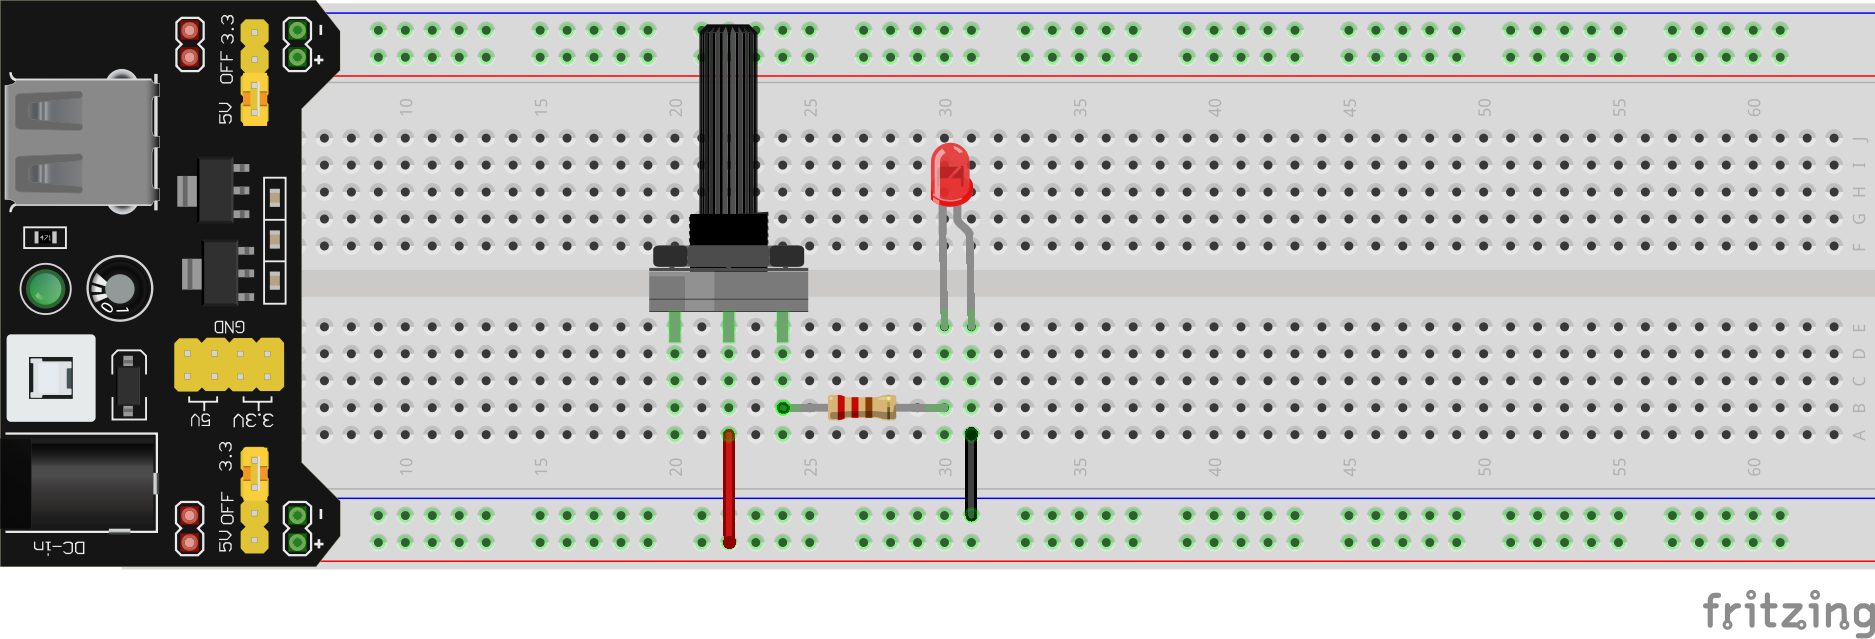
\includegraphics[width=0.8\textwidth]{lesson_circuits/L3/lesson_3.png}
    \caption{Breadboard Schematic}
    \label{fig:pot_led_sch}
\end{figure}
\begin{figure}[!htp]
    \centering
    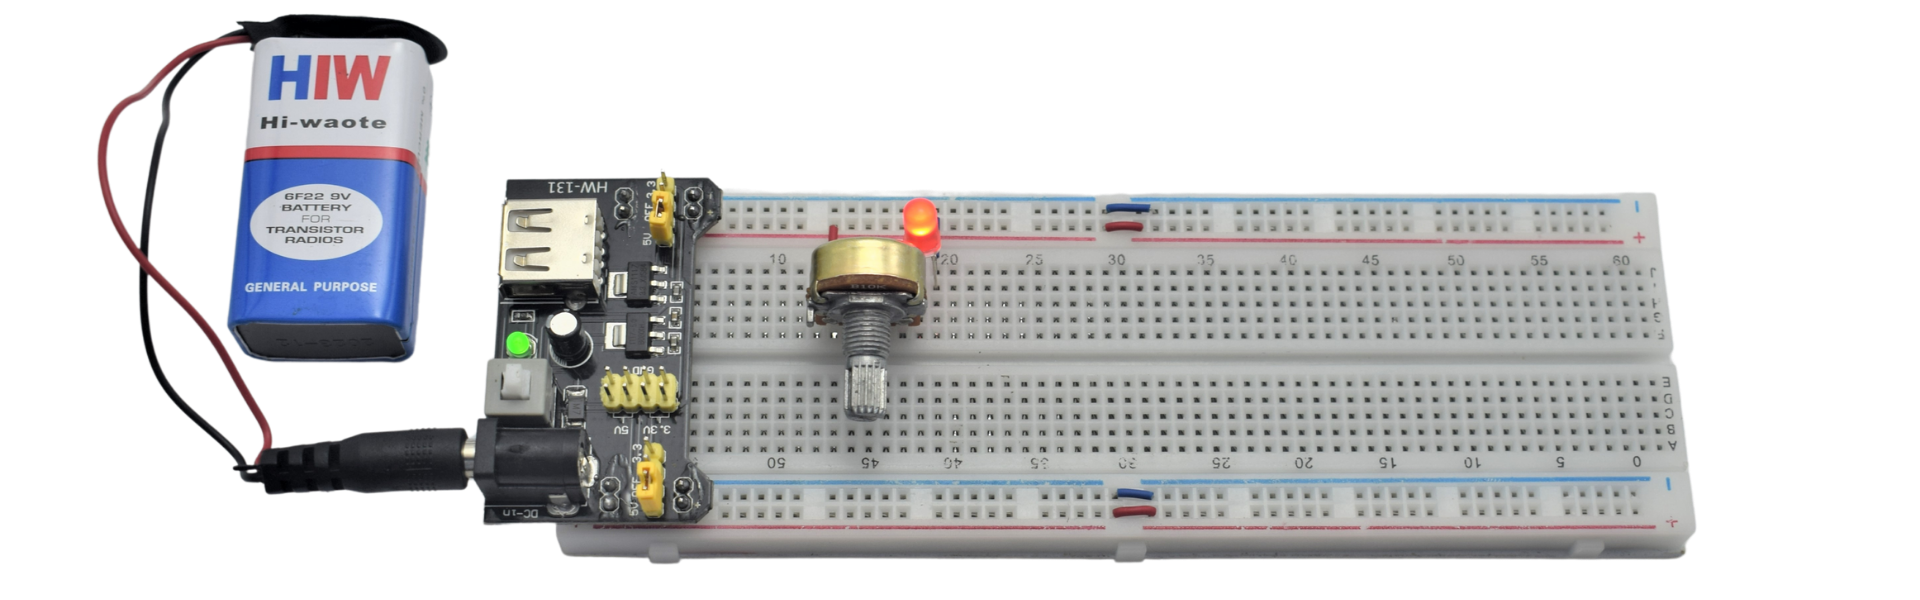
\includegraphics[width=\textwidth]{lesson_circuits/L3/L3-A.png}
    \caption{Max Intensity, $R_{pot} = 0$}
    \label{fig:pot_led_max}
\end{figure}
\begin{figure}[!htp]
    \centering
    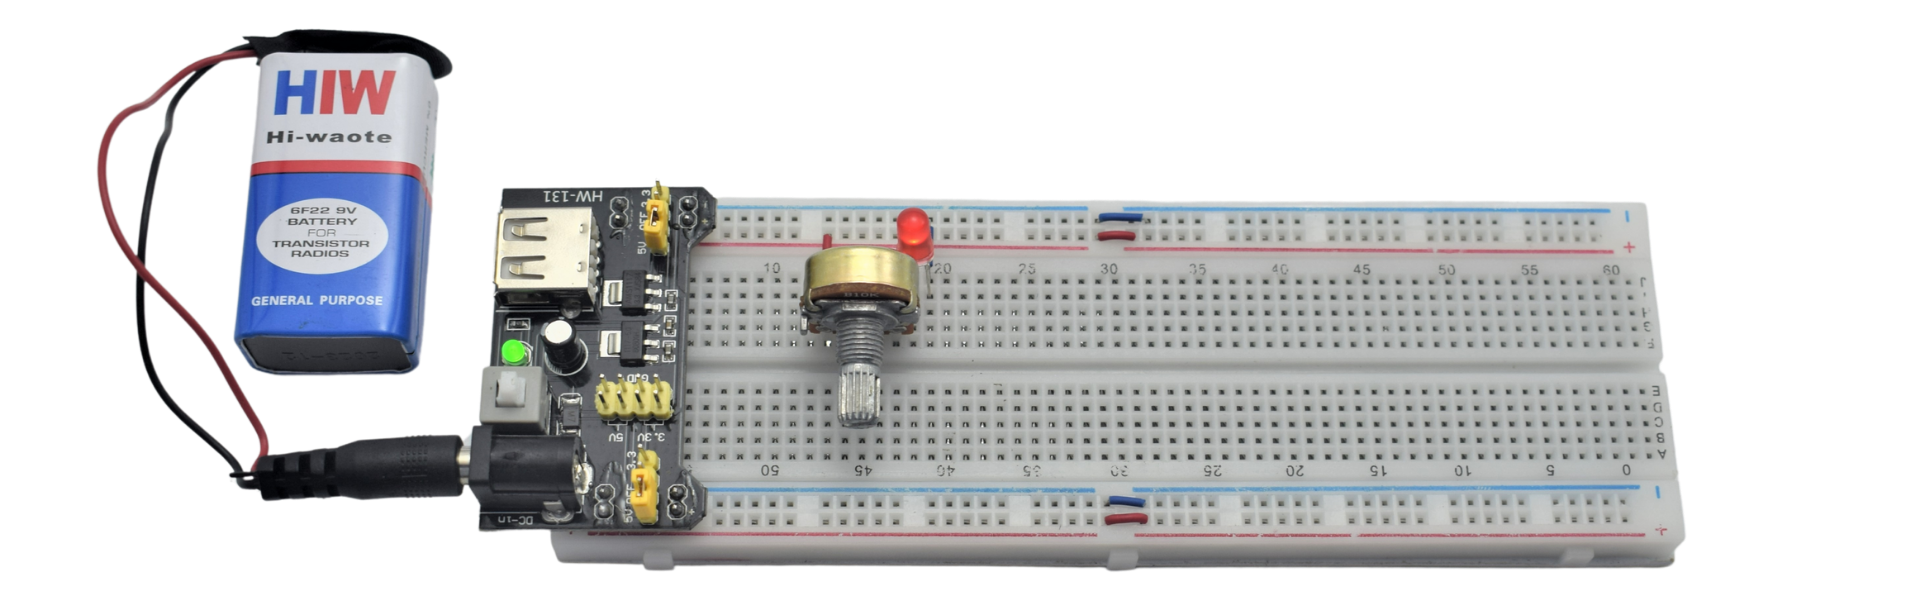
\includegraphics[width=\textwidth]{lesson_circuits/L3/L3-B.png}
    \caption{Min Intensity, $R_{pot} = 10\si{\kilo\ohm}$}
    \label{fig:pot_led_min}
\end{figure}


